\chapter{Návrh riešenia}

\section{Meranie hĺbky pamäte samorganizujúcich sa máp}
Ako trénovaciu množinu budem používať sekvenciu písmen abecedy (26 písmen) zostavenú nenáhodným spôsobom (napr. tvoriacu anglické slová z nejakého korpusu).
Vstupmi (trénovacie príklady) pre sieť budú zakódované jednotlivé písmená z trénovacej sekvencie.
Písmená kódujem do 26 prvkového vektora, ktorého prvky budú nuly a jednotka (pre každé písmeno na inej pozícii).
Každý neurón bude mať množinu, v~ktorej si bude pamätať pre aký vstup bol víťazom. Nebude si však ukladať iba konkrétne písmeno zo vstupu, ale $k$ posledných písmen z trénovacej množiny (tzv. sliding window). 
Z toho si viem ďalej vytvoriť hitmapu, ktorá mi bude vizualizovať, na aké vstupy neuróny reagovali.

\begin{figure}[H]
	\centering
	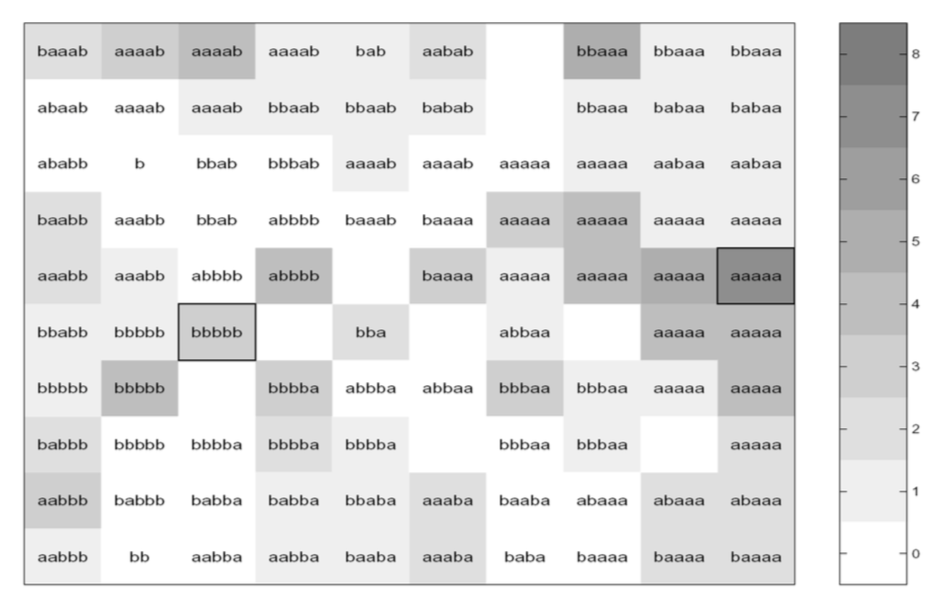
\includegraphics[width=10cm]{assets/receptive_field}
	\caption{Hitmapa}
\end{figure}

Mierou hĺbky pamäte mapy bude potom vážený priemer dĺžky najdlhších spoločných podpostupností písmen v množinách jednotlivých neurónov. Dĺžku najdlhšej podpostupnosti budem určovať od konca sekvencií v množine. Priemer pamäťových hĺbok jednotlivých neurónov musí byť vážený, aby neuróny, %s väčším počtom víťazov mali vyššiu váhu ako neuróny s menším počtom víťazov.
ktoré zvíťazili pre viac vstupov, mali vyššiu váhu ako víťazné neuróny pre menší počet vstupov.
Po každej trénovacej epoche (prechode trénovacou množinou) budem vedieť určiť pamäťovú hĺbku mapy.
Vďaka tomu, že neuróny rekurentných sietí majú okrem normálnych váh aj kontextové váhy, ktoré uchovávajú informáciu z predchádzajúceho kroku,  môže sa stať, že rovnaké písmeno zo vstupu bude mať rôzne víťazné neuróny počas trénovania.

Samotná pamäťová hĺbka je relatívna a závisí od veľkosti sliding window.

Počet neurónov v mape volíme podľa množstva rôznych slov v použitej trénovacej
množine.

Tradeoff medzi rozlišovaciou schopnosťou jednotlivých slov a schopnosťou
zachovať podobné slová topologicky čo najbližšie pri sebe.

Na trénovanie a vyhodnocovanie pamäťovej hĺbky som si vytvoril 3 sady 
trénovacích príkladov. 
Prvá sada sú najednoduchšie sekvenice (slová), ktoré obsahujú veľké množstvo regularít a malé množstvo rôznych písmen.
Napríklad sekvencie ako $aaabbb$,  $bbbaaaaa$.
Druhou sadou budú slová generované Reberovým automatom.
Treťou sadou trénovacích príkladov budú najzložitejšie sekvencie, resp. náhodný text s
veľkým množstvom rôznych písmen. Túto sadu budem používať ako performance benchmark. 

\section{mSOM s leaky integration contextom}
Pre potreby testovania pamäťovej hĺbky sme si vytvorili modifikovanú verziu mSOM, ktorá používa iný kontext.
V pôvodnej mSOM bol kontext tvorený vlastnosťami víťazného neurónu z predchádzajúceho kroku.
V našej modifikovanej verzii mSOM budú kontext tvoriť samotné vstupné vektory z predchádzajúcich krokov.
Všetko ostatné zostane rovnaké ako v pôvodnej mSOM.

Samotný kontext budem počítať pomocou nasledujúceho rekurzívneho vzťahu:
\begin{equation}
	c = \beta^{0} \cdot x_{t} + \beta^{1} \cdot x_{t-1} + 
	\beta^{2} \cdot x_{t-2}....
\end{equation}

$\beta$ parameter je číslo $\beta < 1$

Tým zabezpečím, že kontext bude tvorený nejakou lineárnou kombináciou 
predchádzajúcich vstupov a čím ďalej idem do minulosti, tým majú tieto vstupy 
menšiu váhu (vďaka umocňovaniu beta parametra). 




